\documentclass[12pt,a4paper]{report}

\usepackage[utf8]{inputenc}
\usepackage[T1]{fontenc}
\usepackage[italian]{babel}
\usepackage{amsmath}
\usepackage{graphicx}
\usepackage{float}
\usepackage{hyperref}
\usepackage{setspace}
\usepackage{array}
\usepackage[a4paper, margin=2.5cm]{geometry}
\usepackage{amssymb}
\usepackage{qrcode}
\usepackage{placeins}


\hypersetup{
    colorlinks=true,
    linkcolor=black,
    urlcolor=blue
}

\begin{document}

% ------------------ TITLE PAGE ------------------
\begin{titlepage}
\centering

\vspace*{0.5cm}


\includegraphics[width=0.5\textwidth]{logo_unical.png}

\vspace{0.8cm}

{\Large \textbf{University of Calabria}\par}

\vspace{0.25cm}

{\large Department of Computer Engineering, Modelling, Electronics\\
and Systems Engineering (DIMES)\par}

\vspace{0.25cm}

{\large MSc in Robotics and Automation Engineering\par}

\vspace{3.2cm}

{\Large \textbf{Design and Analysis of Reinforcement Learning Agents in a Pac-Man Environment}\par}

\vspace{3.2cm}

\begin{center}
\begin{minipage}{0.42\textwidth}
\raggedright
\textbf{Course:}\\
Intelligent Systems for Robotics

\vspace{0.4cm}

\textbf{Instructor:}\\
Prof. Francesco Pupo
\end{minipage}
\hfill
\begin{minipage}{0.20\textwidth}
\raggedright
\textbf{Student:}\\
Ludovica Perroni

\vspace{0.4cm}

\textbf{Student ID:}\\
269200
\end{minipage}
\end{center}

\vfill

{\large Academic Year 2025--2026\par}

\end{titlepage}

% ------------------ TABLE OF CONTENTS ------------------
\renewcommand{\contentsname}{Indice}
\tableofcontents
\newpage

\begin{abstract}

Questo progetto presenta lo sviluppo di un ambiente semplificato ispirato al gioco Pac-Man per lo studio di algoritmi di Reinforcement Learning. In particolare, vengono implementati e confrontati due algoritmi tabulari: Q-Learning e SARSA. L’agente controlla Pac-Man all’interno di una griglia bidimensionale, con l’obiettivo di raccogliere cibo evitando la collisione con un fantasma.

L’ambiente include elementi di stochasticità, dovuti sia al movimento del fantasma sia alla generazione casuale del cibo, rendendo il problema adatto all’apprendimento tramite interazione con l’ambiente. Durante il training gli agenti apprendono una politica decisionale utilizzando una strategia epsilon-greedy e una funzione di reward progettata per incentivare la sopravvivenza e la raccolta del cibo.

Le prestazioni ottenute vengono confrontate con quelle di un agente casuale utilizzando diverse metriche, tra cui reward media, numero medio di cibi raccolti, numero medio di step sopravvissuti e collision rate. I risultati mostrano che entrambi gli algoritmi di Reinforcement Learning riescono ad apprendere strategie efficaci, superando nettamente il comportamento casuale. Inoltre, il confronto evidenzia differenze coerenti con la teoria tra l’approccio off-policy del Q-Learning e quello on-policy di SARSA.

\end{abstract}

\chapter{Introduzione}

Il Reinforcement Learning (RL) rappresenta una delle principali tecniche di apprendimento automatico utilizzate per la risoluzione di problemi decisionali sequenziali. A differenza dell’apprendimento supervisionato, in cui il modello apprende a partire da esempi etichettati, nel Reinforcement Learning un agente impara attraverso l’interazione diretta con un ambiente. Durante questo processo, l’agente osserva uno stato, seleziona un’azione e riceve una ricompensa che valuta la qualità della decisione presa. L’obiettivo è apprendere una politica ottimale in grado di massimizzare la reward cumulativa nel lungo termine.

Negli ultimi anni il Reinforcement Learning ha trovato applicazione in numerosi ambiti, tra cui robotica, videogiochi, sistemi autonomi e controllo intelligente. In particolare, i videogiochi rappresentano un contesto ideale per lo studio di algoritmi RL, poiché richiedono pianificazione, adattamento dinamico e gestione di obiettivi multipli.

In questo progetto viene sviluppato un ambiente semplificato ispirato al gioco Pac-Man. L’agente controlla Pac-Man all’interno di una griglia bidimensionale e deve raccogliere cibo evitando la collisione con un fantasma. Il problema presenta elementi di stochasticità, dovuti sia alla generazione casuale del cibo sia al comportamento non deterministico del fantasma, rendendo necessario l’apprendimento di strategie adattive.

Lo scopo del progetto è confrontare il comportamento di due algoritmi classici di Reinforcement Learning tabulare: Q-Learning e SARSA. Entrambi gli algoritmi utilizzano una Q-table per stimare il valore delle azioni nei diversi stati dell’ambiente, ma differiscono nella modalità di aggiornamento dei valori Q. Il confronto permette di evidenziare le differenze tra un approccio off-policy, rappresentato dal Q-Learning, e un approccio on-policy, rappresentato da SARSA.

Le prestazioni degli agenti vengono valutate confrontandole con quelle di un agente casuale attraverso diverse metriche, tra cui reward media, numero di cibi raccolti, numero medio di step sopravvissuti e tasso di collisione con il fantasma. Inoltre, vengono analizzati i grafici di training per osservare l’evoluzione dell’apprendimento durante gli episodi.

L’obiettivo finale del progetto è verificare la capacità degli algoritmi di Reinforcement Learning di apprendere strategie efficaci in un ambiente dinamico e parzialmente stocastico, evidenziandone punti di forza e differenze comportamentali.

\begin{figure}[H]
    \centering
    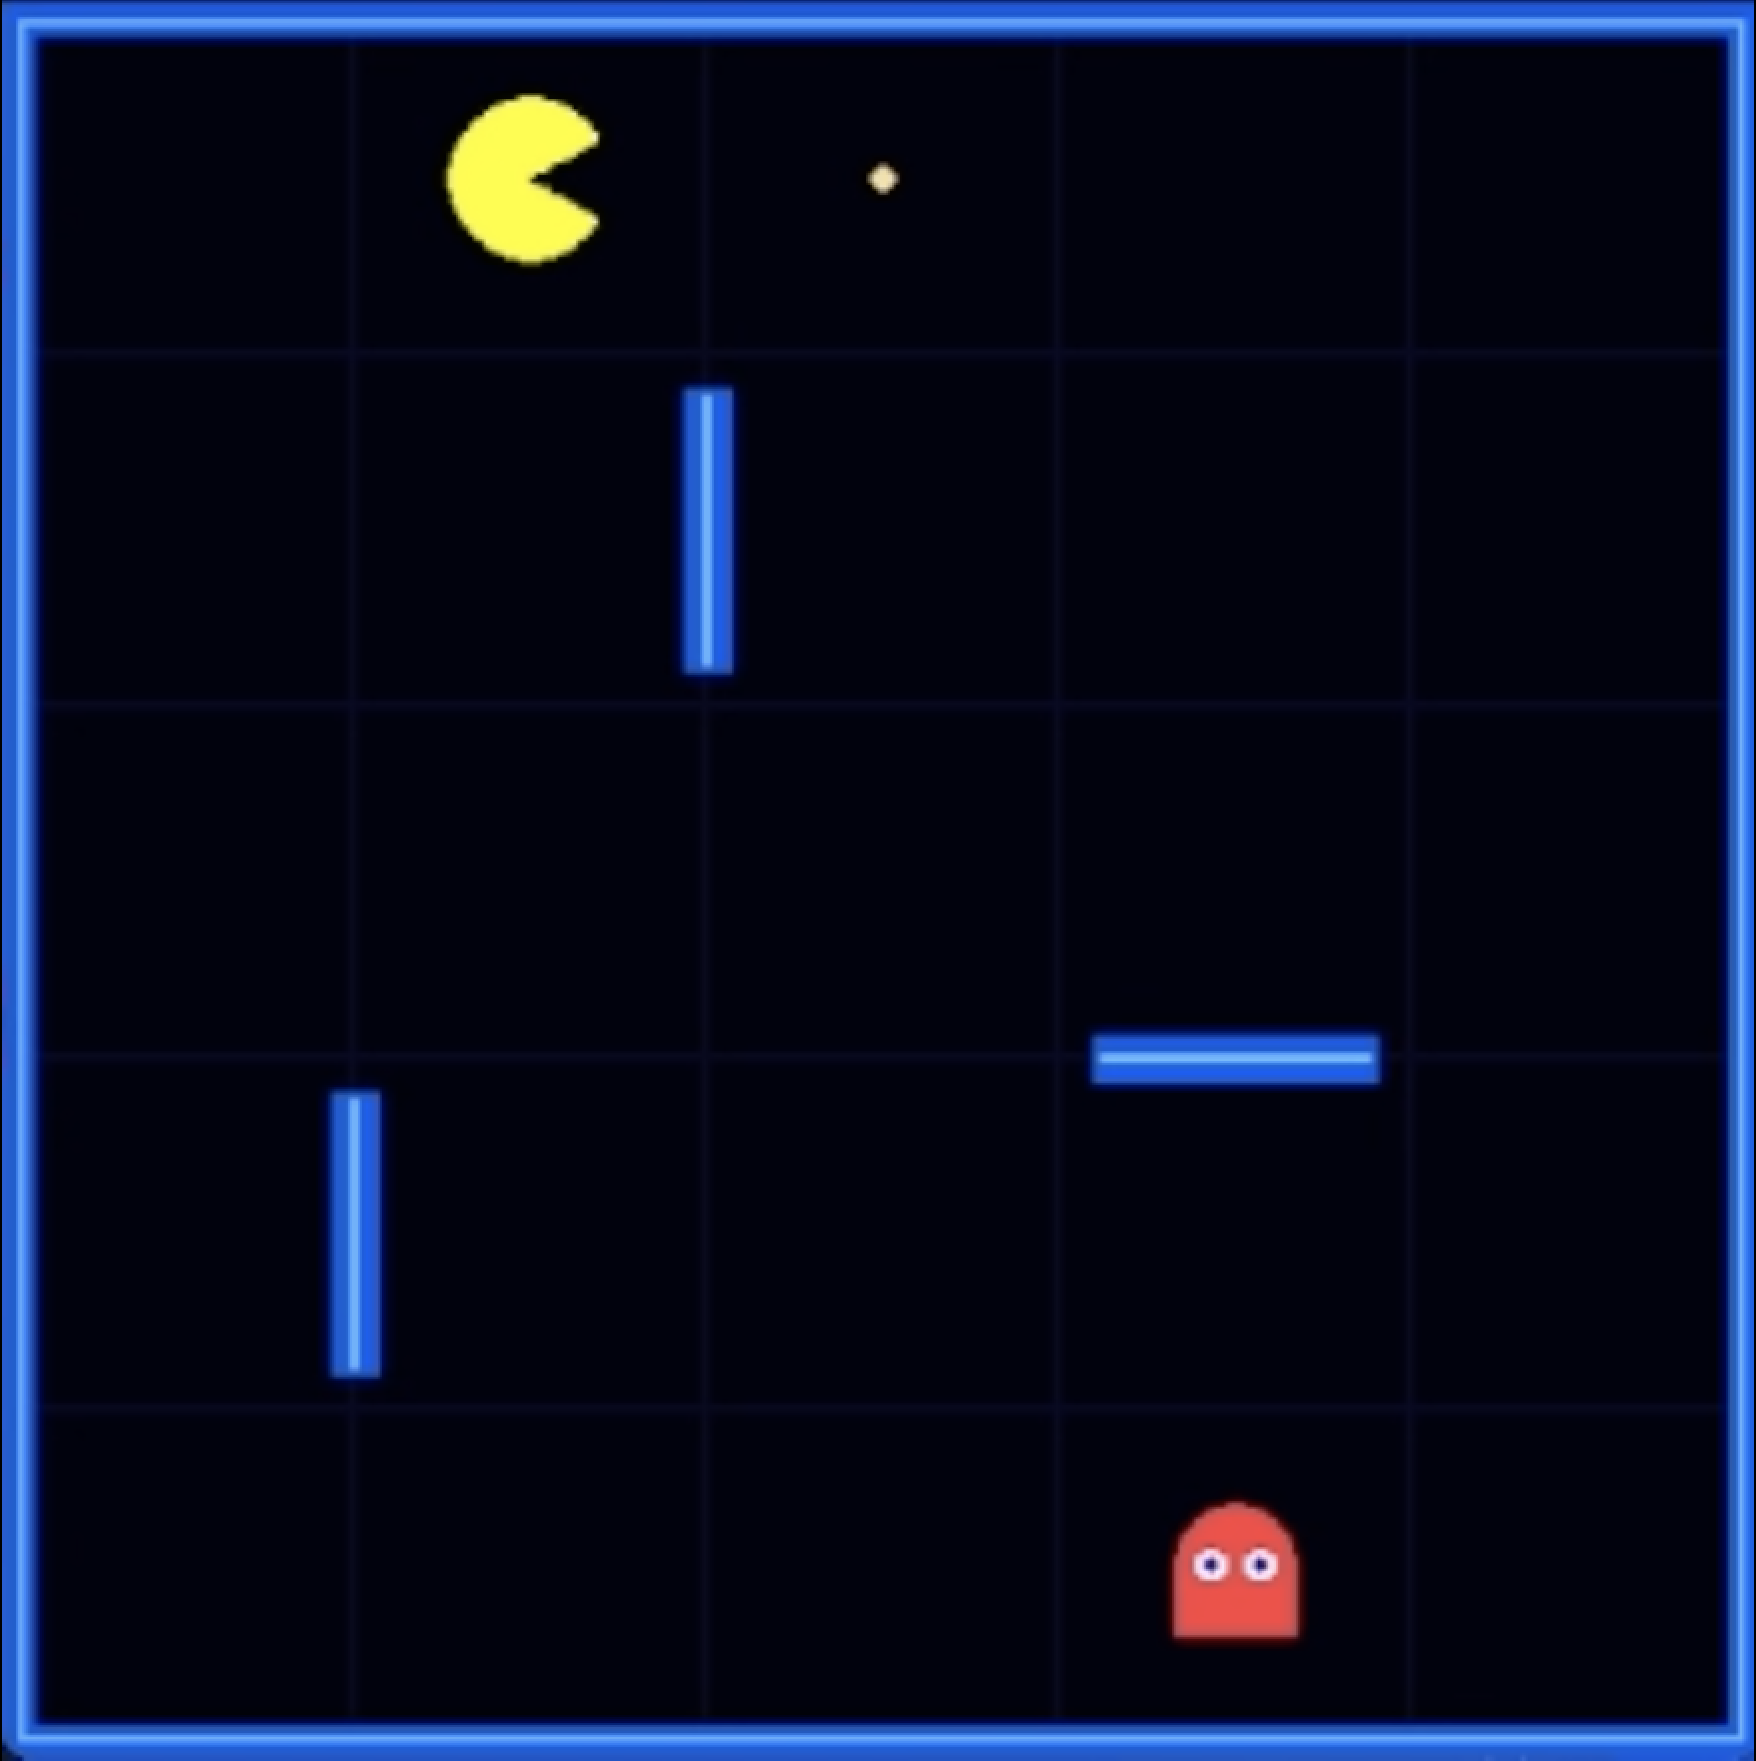
\includegraphics[width=0.55\textwidth]{pacman_environment.png}
    \caption{Ambiente Pac-Man utilizzato per l’addestramento degli agenti di Reinforcement Learning.}
    \label{fig:pacman_environment}
\end{figure}

\FloatBarrier

La Figura~\ref{fig:pacman_environment} mostra l’ambiente sviluppato per il progetto. L’agente Pac-Man deve raccogliere il cibo evitando il fantasma all’interno della griglia contenente ostacoli.


\chapter{Descrizione dell’Ambiente}

L’ambiente sviluppato per questo progetto rappresenta una versione semplificata del gioco Pac-Man, progettata specificamente per lo studio di algoritmi di Reinforcement Learning. L’ambiente è implementato come una griglia bidimensionale di dimensione $5 \times 5$, all’interno della quale interagiscono tre elementi principali: Pac-Man, il fantasma e il cibo.

\section{Struttura della griglia}

La griglia è composta da 25 celle. Pac-Man parte sempre dalla posizione in alto a sinistra, mentre il fantasma parte dalla posizione in basso a destra. Il cibo viene invece generato casualmente all’inizio di ogni episodio in una posizione valida diversa da quelle occupate dagli altri elementi.

All’interno della griglia sono inoltre presenti alcuni muri che impediscono il passaggio diretto tra determinate celle. La presenza dei muri aumenta la complessità del problema, poiché limita i movimenti disponibili e obbliga l’agente a pianificare percorsi alternativi.

\section{Rappresentazione dello stato}

Lo stato dell’ambiente è rappresentato attraverso una tupla composta dalle coordinate di Pac-Man, del cibo e del fantasma:

\begin{equation}
s = (p_r, p_c, f_r, f_c, g_r, g_c)
\end{equation}

dove:

\begin{itemize}
    \item $(p_r,p_c)$ rappresenta la posizione di Pac-Man;
    \item $(f_r,f_c)$ rappresenta la posizione del cibo;
    \item $(g_r,g_c)$ rappresenta la posizione del fantasma.
\end{itemize}

Questa rappresentazione permette all’agente di osservare completamente l’ambiente in ogni istante.

\section{Azioni disponibili}

L’agente può eseguire quattro azioni:

\begin{itemize}
    \item movimento verso l’alto;
    \item movimento verso il basso;
    \item movimento verso sinistra;
    \item movimento verso destra.
\end{itemize}

Un movimento viene considerato valido solo se:

\begin{itemize}
    \item rimane all’interno della griglia;
    \item non attraversa un muro.
\end{itemize}

In caso di movimento non valido, Pac-Man rimane nella posizione corrente e riceve una penalità.

\section{Movimento del fantasma}

Il fantasma utilizza una strategia semi-stocastica. Con probabilità del 70\% si muove cercando di avvicinarsi a Pac-Man, mentre con probabilità del 30\% effettua un movimento casuale tra quelli validi.

Questa scelta rende l’ambiente non completamente deterministico, poiché la stessa azione eseguita da Pac-Man può produrre risultati differenti a seconda del comportamento del fantasma.

\section{Condizioni di terminazione}

Ogni episodio termina quando si verifica una delle seguenti condizioni:

\begin{itemize}
    \item Pac-Man entra in collisione con il fantasma;
    \item viene raggiunto il numero massimo di step consentiti.
\end{itemize}

Nel progetto il numero massimo di step per episodio è stato fissato a 100.

\chapter{Funzione di Reward}

La progettazione della funzione di reward rappresenta uno degli aspetti più importanti nel Reinforcement Learning, poiché influenza direttamente il comportamento appreso dall’agente. In questo progetto è stata definita una funzione di reward con l’obiettivo di incentivare Pac-Man a raccogliere il cibo, sopravvivere il più a lungo possibile ed evitare il fantasma.

\section{Reward per ogni step}

A ogni azione eseguita viene applicata una penalità base pari a:

\begin{equation}
r = -1
\end{equation}

Questa penalità ha lo scopo di scoraggiare movimenti inutili e incentivare l’agente a raggiungere rapidamente il cibo.

\section{Movimenti non validi}

Se Pac-Man tenta di attraversare un muro oppure uscire dai limiti della griglia, il movimento viene considerato non valido e viene applicata una penalità aggiuntiva:

\begin{equation}
r = -5
\end{equation}

In questo caso Pac-Man rimane nella stessa posizione.

\section{Reward shaping basato sulla distanza}

Per accelerare l’apprendimento è stata introdotta una strategia di reward shaping basata sulla distanza di Manhattan tra Pac-Man e il cibo.

La distanza di Manhattan è definita come:

\begin{equation}
d = |p_r - f_r| + |p_c - f_c|
\end{equation}

Se dopo una mossa Pac-Man si avvicina al cibo, viene assegnato un bonus:

\begin{equation}
r = r + 1
\end{equation}

Se invece si allontana dal cibo, viene applicata una penalità:

\begin{equation}
r = r - 1
\end{equation}

Questa tecnica fornisce feedback più frequenti all’agente e facilita l’apprendimento di comportamenti utili anche nelle prime fasi del training.

\section{Raccolta del cibo}

Quando Pac-Man raggiunge la posizione del cibo, riceve una reward positiva:

\begin{equation}
r = r + 10
\end{equation}

Successivamente il cibo viene rigenerato casualmente in una nuova posizione valida della griglia.

\section{Collisione con il fantasma}

Se Pac-Man entra in collisione con il fantasma, l’episodio termina immediatamente e viene assegnata una penalità elevata:

\begin{equation}
r = -50
\end{equation}

Questa scelta permette all’agente di apprendere rapidamente che la collisione rappresenta un evento fortemente negativo da evitare.

\section{Considerazioni sulla reward}

La funzione di reward progettata combina penalità e ricompense con l’obiettivo di guidare gradualmente l’agente verso comportamenti efficaci. In particolare:

\begin{itemize}
    \item le penalità per step incentivano percorsi brevi;
    \item il reward shaping accelera l’apprendimento;
    \item la reward positiva per il cibo incentiva il raggiungimento dell’obiettivo;
    \item la forte penalità per collisione favorisce strategie di sopravvivenza.
\end{itemize}

L’utilizzo del reward shaping si è rivelato particolarmente utile per stabilizzare il training e rendere più evidente il miglioramento delle performance durante gli episodi.

\chapter{Algoritmi di Reinforcement Learning}

Per risolvere il problema proposto sono stati implementati due algoritmi classici di Reinforcement Learning tabulare: Q-Learning e SARSA. Entrambi utilizzano una Q-table per memorizzare il valore associato a ciascuna coppia stato-azione, ma differiscono nel modo in cui aggiornano tali valori durante il training.

\section{Q-Table}

La Q-table rappresenta una struttura dati che associa a ogni stato dell’ambiente un insieme di valori Q, uno per ciascuna azione possibile. Il valore Q di una coppia $(s,a)$ rappresenta una stima della reward cumulativa futura ottenibile eseguendo l’azione $a$ nello stato $s$.

Formalmente:

\begin{equation}
Q(s,a) = \text{reward futura attesa eseguendo } a \text{ nello stato } s
\end{equation}

Durante il training la Q-table viene aggiornata progressivamente in base alle esperienze raccolte dall’agente.

\section{Politica \texorpdfstring{$\epsilon$}{epsilon}-greedy}

Entrambi gli algoritmi utilizzano una politica $\epsilon$-greedy per bilanciare esplorazione e sfruttamento.

Con probabilità $\epsilon$ l’agente seleziona un’azione casuale, esplorando nuove possibilità. Con probabilità $1-\epsilon$, invece, seleziona l’azione con valore Q massimo nello stato corrente.

Formalmente:

\begin{equation}
a =
\begin{cases}
\text{azione casuale} & \text{con probabilità } \epsilon \\
\arg\max_a Q(s,a) & \text{con probabilità } 1-\epsilon
\end{cases}
\end{equation}

Nel progetto è stato utilizzato un valore costante:

\begin{equation}
\epsilon = 0.1
\end{equation}

\section{Q-Learning}

Il Q-Learning è un algoritmo off-policy. Questo significa che l’aggiornamento della Q-table viene effettuato assumendo che, nello stato successivo, venga scelta l’azione ottimale, indipendentemente dalla politica realmente utilizzata durante l’esplorazione.

La regola di aggiornamento è:

\begin{equation}
Q(s,a) \leftarrow Q(s,a) +
\alpha \left[
r + \gamma \max_{a'} Q(s',a') - Q(s,a)
\right]
\end{equation}

dove:

\begin{itemize}
    \item $\alpha$ rappresenta il learning rate;
    \item $\gamma$ rappresenta il discount factor;
    \item $r$ è la reward ricevuta;
    \item $s'$ è lo stato successivo.
\end{itemize}

Il termine:

\begin{equation}
\max_{a'} Q(s',a')
\end{equation}

rappresenta la migliore reward futura stimata nello stato successivo.

Grazie a questa caratteristica, il Q-Learning tende a sviluppare strategie più aggressive e orientate alla massimizzazione della reward.

\section{SARSA}

SARSA è invece un algoritmo on-policy. A differenza del Q-Learning, aggiorna la Q-table utilizzando il valore dell’azione effettivamente scelta dalla politica corrente nello stato successivo.

La regola di aggiornamento è:

\begin{equation}
Q(s,a) \leftarrow Q(s,a) +
\alpha \left[
r + \gamma Q(s',a') - Q(s,a)
\right]
\end{equation}

In questo caso, l’aggiornamento dipende direttamente dall’azione realmente eseguita nel passo successivo.

Poiché SARSA tiene conto anche delle azioni esplorative introdotte dalla politica $\epsilon$-greedy, tende generalmente ad apprendere strategie più conservative rispetto al Q-Learning.

\section{Differenze tra Q-Learning e SARSA}

La principale differenza tra i due algoritmi riguarda il modo in cui stimano il valore futuro.

\begin{itemize}
    \item Q-Learning utilizza il massimo valore Q possibile nello stato successivo, assumendo sempre una scelta ottimale.
    \item SARSA utilizza il valore dell’azione effettivamente scelta dalla politica corrente.
\end{itemize}

Di conseguenza:

\begin{itemize}
    \item Q-Learning tende a essere più ottimista e aggressivo;
    \item SARSA tende a essere più prudente e stabile.
\end{itemize}

Nel contesto del progetto, questa differenza si riflette nelle performance finali degli agenti e nel loro comportamento durante il training.

\chapter{Implementazione del Progetto}

Il progetto è stato sviluppato interamente in Python, utilizzando diverse librerie per la gestione dell’ambiente, dell’addestramento degli agenti e della visualizzazione grafica.

\section{Tecnologie utilizzate}

Le principali librerie utilizzate sono:

\begin{itemize}
    \item \textbf{NumPy}: utilizzata per la gestione della Q-table e delle operazioni numeriche;
    
    \item \textbf{Pygame}: utilizzata per la realizzazione grafica dell’ambiente Pac-Man e per la simulazione interattiva;
    
    \item \textbf{Matplotlib}: utilizzata per la generazione dei grafici di training e dei confronti tra gli agenti;
    
    \item \textbf{JSON e CSV}: utilizzati per il salvataggio dei risultati sperimentali.
\end{itemize}

\section{Struttura del progetto}

Il progetto è organizzato in più file Python, ciascuno dedicato a una specifica funzionalità.

In particolare:

\begin{itemize}
    \item \texttt{environment.py} definisce l’ambiente Pac-Man;
    
    \item \texttt{train\_qlearning.py} implementa l’algoritmo Q-Learning;
    
    \item \texttt{train\_sarsa.py} implementa l’algoritmo SARSA;
    
    \item \texttt{visualizer.py} gestisce la visualizzazione grafica della simulazione;
    
    \item \texttt{save\_results.py} salva grafici e metriche finali;
    
    \item \texttt{main.py} esegue il training e la valutazione degli agenti.
\end{itemize}

\section{Gestione della simulazione}

La simulazione viene eseguita episodicamente. A ogni episodio:

\begin{enumerate}
    \item l’ambiente viene inizializzato;
    \item Pac-Man interagisce con la griglia;
    \item il fantasma si muove secondo una politica semi-stocastica;
    \item l’agente aggiorna la Q-table;
    \item vengono salvate le metriche di training.
\end{enumerate}

Durante la fase finale del progetto è stata inoltre implementata una visualizzazione grafica in tempo reale, utile per osservare qualitativamente il comportamento degli agenti addestrati.


\chapter{Training degli Agenti}

Il processo di training consiste nell’interazione ripetuta tra l’agente e l’ambiente. Durante ogni episodio, Pac-Man osserva lo stato corrente, seleziona un’azione tramite la politica $\epsilon$-greedy e aggiorna la Q-table in base alla reward ricevuta e allo stato successivo.

\section{Parametri di training}

Entrambi gli algoritmi sono stati addestrati utilizzando gli stessi parametri, in modo da rendere il confronto il più possibile equo.

I parametri utilizzati sono riportati nella Tabella~\ref{tab:parametri_training}.

\begin{table}[H]
\centering
\begin{tabular}{lc}
\hline
Parametro & Valore \\
\hline
Numero di episodi & 10000 \\
Learning rate $\alpha$ & 0.1 \\
Discount factor $\gamma$ & 0.95 \\
Epsilon $\epsilon$ & 0.1 \\
Step massimi per episodio & 100 \\
\hline
\end{tabular}
\caption{Parametri utilizzati durante il training.}
\label{tab:parametri_training}
\end{table}

\section{Monitoraggio del training}

Durante il training sono state salvate diverse informazioni per monitorare l’apprendimento degli agenti:

\begin{itemize}
    \item reward totale ottenuta in ogni episodio;
    \item media cumulativa delle reward;
    \item media mobile delle reward;
    \item andamento del valore Q associato allo stato iniziale.
\end{itemize}

La media cumulativa permette di osservare il miglioramento complessivo dell’agente nel corso degli episodi, mentre la media mobile consente di ridurre il rumore presente nella reward dei singoli episodi e rendere più leggibile il trend generale.

\section{Andamento del training di Q-Learning}

La Figura~\ref{fig:qlearning_training} mostra l’andamento del training dell’agente Q-Learning.

\begin{figure}[H]
    \centering
    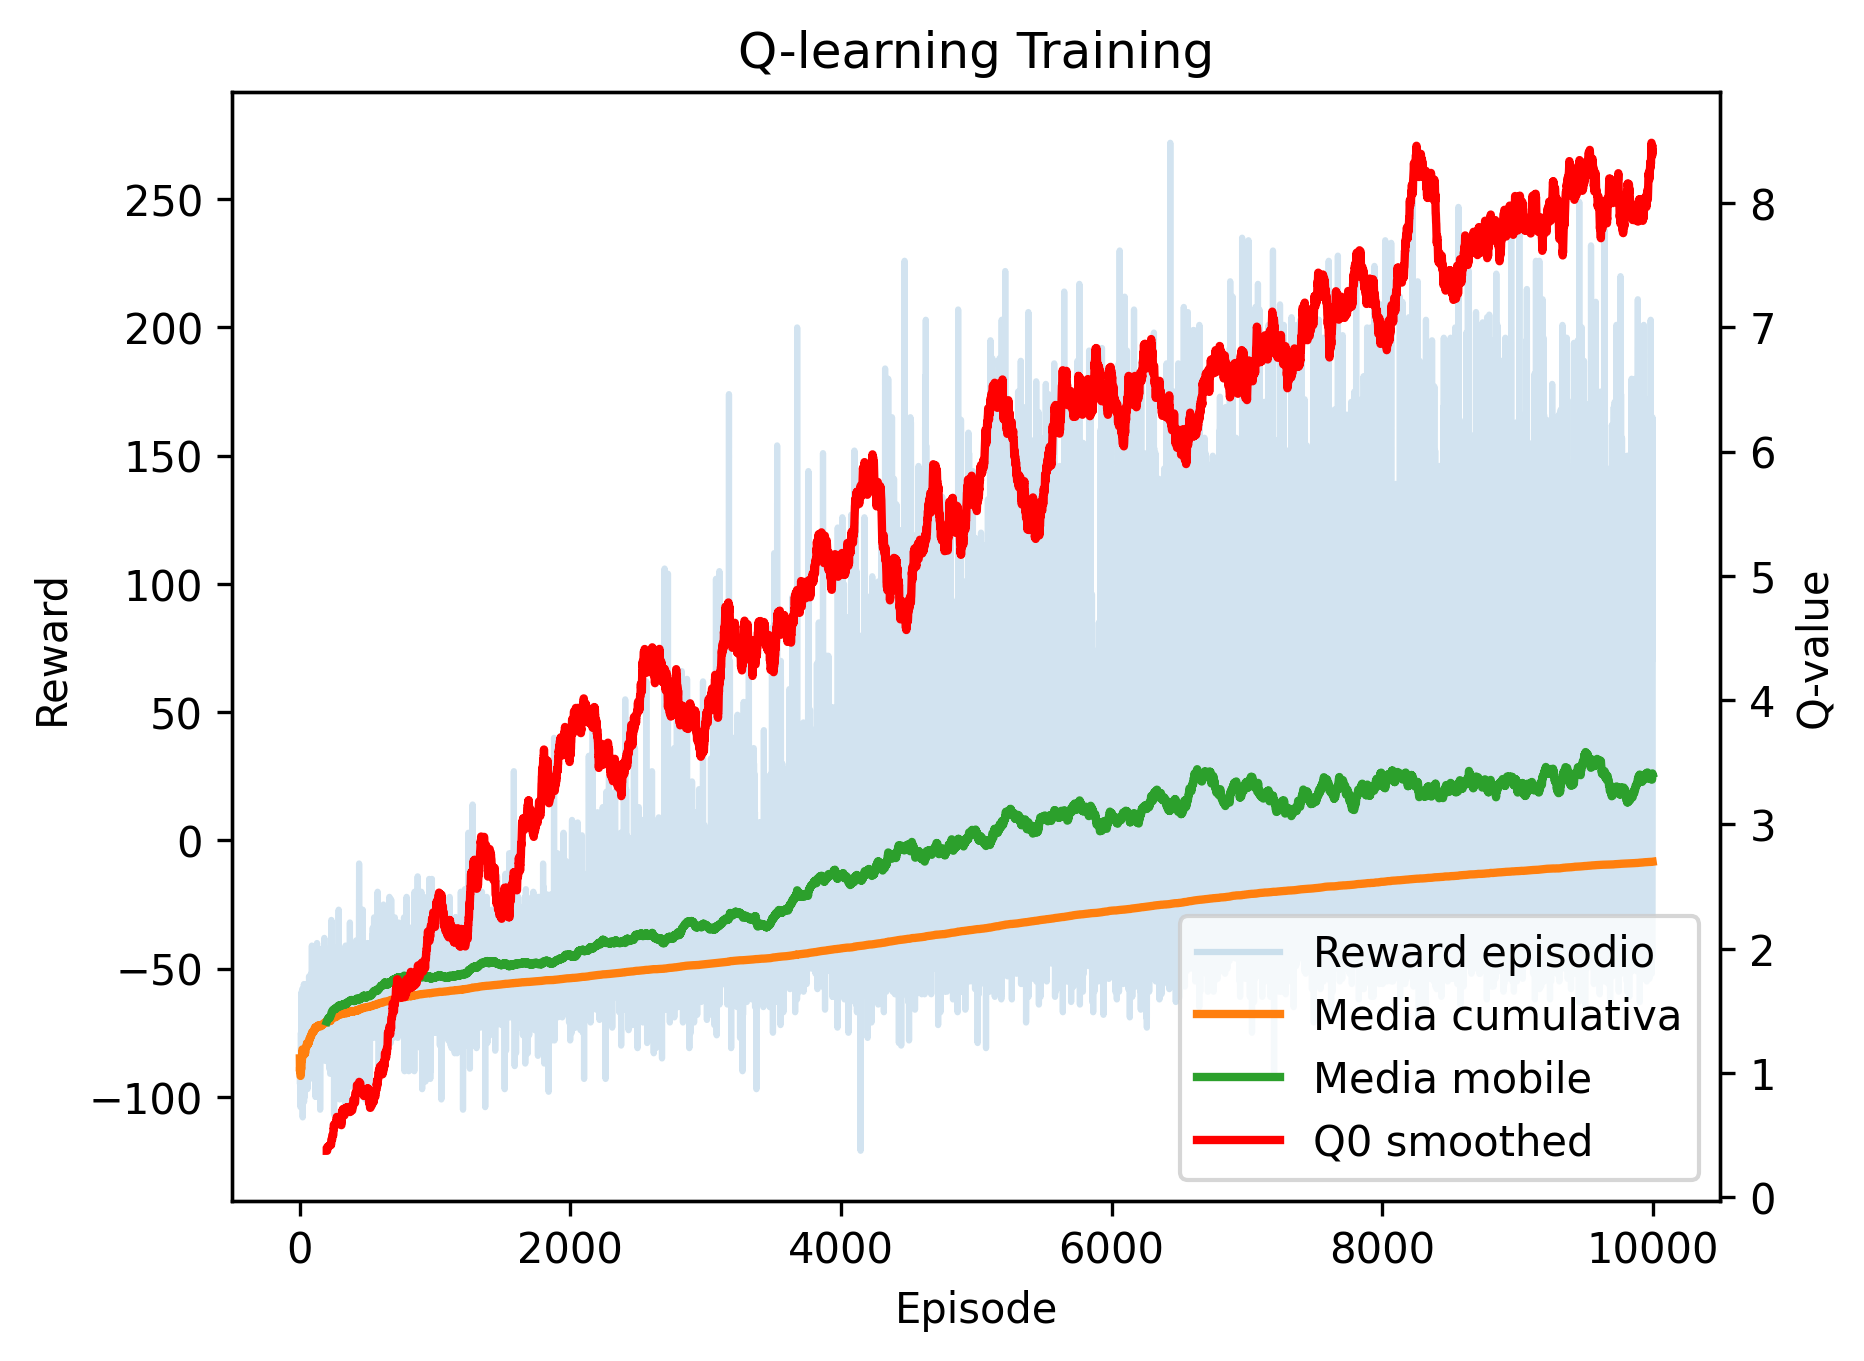
\includegraphics[width=0.9\textwidth]{qlearning_training.png}
    \caption{Andamento della reward e del Q-value durante il training dell’agente Q-Learning}
    \label{fig:qlearning_training}
\end{figure}

\FloatBarrier

Nel grafico è possibile osservare che:

\begin{itemize}
    \item la reward dei singoli episodi presenta un andamento molto rumoroso;
    \item la media cumulativa cresce progressivamente;
    \item la media mobile mostra un miglioramento evidente delle performance;
    \item il valore Q dello stato iniziale tende ad aumentare durante il training.
\end{itemize}

L’elevata variabilità della reward è dovuta alla natura stocastica dell’ambiente. In particolare, la posizione del cibo cambia casualmente a ogni episodio e il fantasma utilizza una politica di movimento parzialmente casuale.

Il valore Q monitorato non converge perfettamente a un valore costante. Questo comportamento è plausibile perché lo stato iniziale dell’episodio non è sempre identico: la posizione del cibo varia casualmente e l’agente continua a esplorare tramite la politica $\epsilon$-greedy. Pertanto, il Q-value deve essere interpretato come un indicatore generale dell’apprendimento della Q-table, piuttosto che come una misura esatta della convergenza.

\section{Andamento del training di SARSA}

La Figura~\ref{fig:sarsa_training} mostra il training dell’agente SARSA.

\begin{figure}[H]
    \centering
    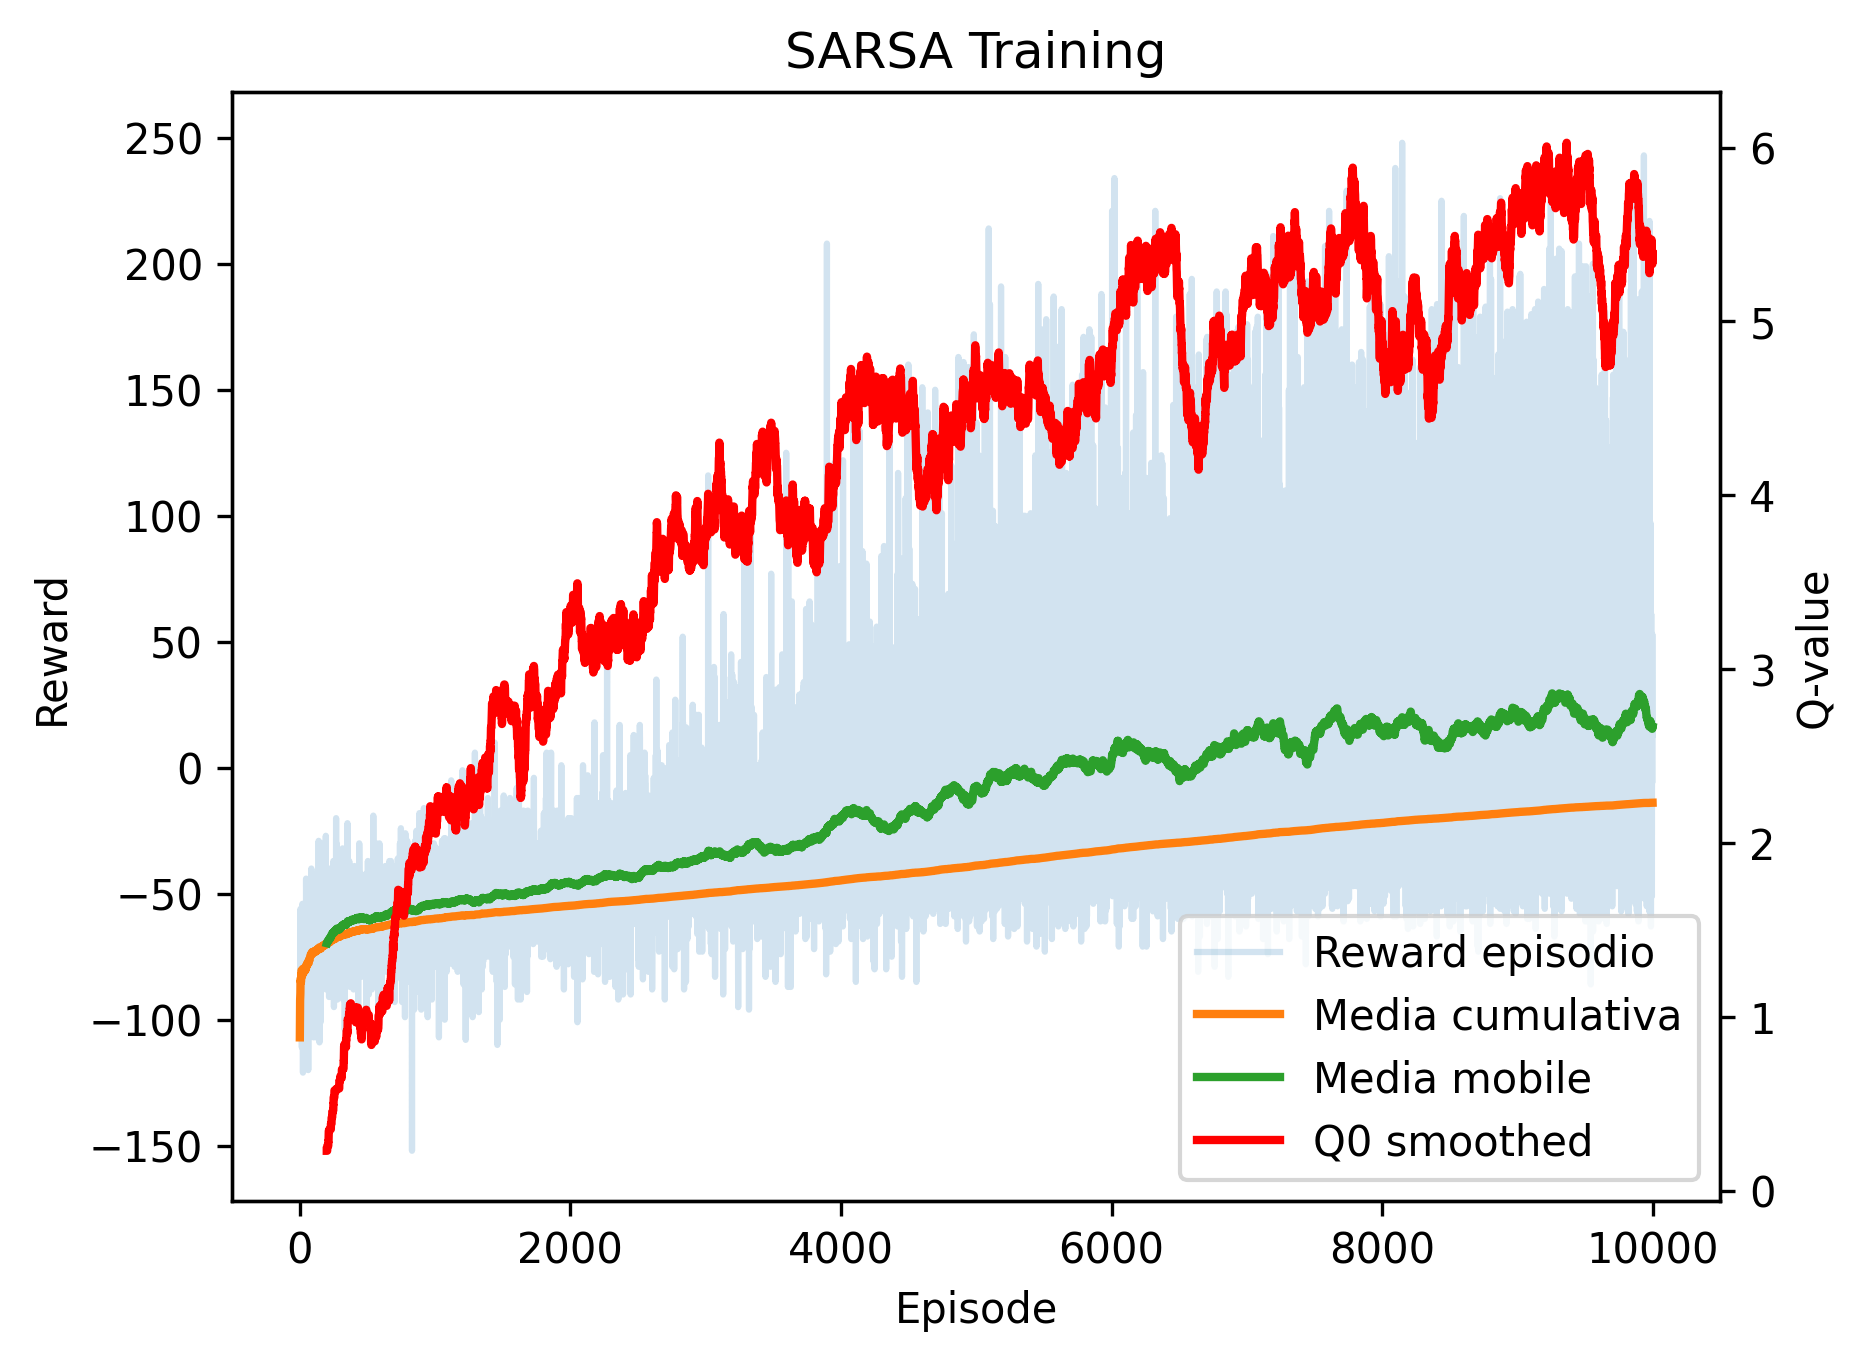
\includegraphics[width=0.9\textwidth]{sarsa_training.png}
    \caption{Andamento della reward e del Q-value durante il training dell’agente SARSA}
    \label{fig:sarsa_training}
\end{figure}

\FloatBarrier
Anche SARSA mostra un miglioramento progressivo delle performance durante il training. La media mobile cresce gradualmente e raggiunge valori elevati nelle fasi finali dell’addestramento.

Rispetto al Q-Learning, SARSA presenta un comportamento leggermente più conservativo. Questo risultato è coerente con la natura on-policy dell’algoritmo, che aggiorna la Q-table considerando le azioni realmente selezionate dalla politica corrente, comprese quelle esplorative.

\section{Considerazioni sul training}

I grafici mostrano che entrambi gli algoritmi riescono ad apprendere strategie efficaci per il problema proposto. L’aumento della reward media e la riduzione delle collisioni durante gli episodi indicano che gli agenti imparano progressivamente a:

\begin{itemize}
    \item evitare il fantasma;
    \item raggiungere rapidamente il cibo;
    \item sopravvivere per un numero elevato di step.
\end{itemize}

Nonostante il rumore presente nei grafici, dovuto alla stochasticità dell’ambiente, il trend generale conferma la presenza di apprendimento.

\section{Video dimostrativo della simulazione}

Per osservare qualitativamente il comportamento degli agenti addestrati, è stato realizzato un video dimostrativo della simulazione dell’ambiente Pac-Man.

Nel video è possibile osservare:
\begin{itemize}
    \item il comportamento dell’agente addestrato tramite Q-Learning;
    \item il comportamento dell’agente addestrato tramite SARSA;
    \item la capacità degli agenti di evitare il fantasma;
    \item la raccolta del cibo durante l’esecuzione.
\end{itemize}

Il video completo è disponibile tramite il seguente QR code:

\begin{center}
\qrcode[height=5cm]{https://raw.githubusercontent.com/ludovicap/Intelligent-Systems-for-Robotics/main/simulazione_video.mov}
\end{center}

\begin{center}
\href{https://github.com/ludovicap/Intelligent-Systems-for-robotics}{Repository GitHub del progetto}
\end{center}

\chapter{Valutazione delle Prestazioni}

Dopo il training, gli agenti Q-Learning e SARSA sono stati valutati eseguendo episodi di test senza apprendimento aggiuntivo. Durante la fase di valutazione gli agenti utilizzano una politica greedy, selezionando sempre l’azione con valore Q massimo nello stato corrente.

Le prestazioni ottenute sono state confrontate con quelle di un agente casuale, che seleziona le azioni in modo completamente randomico.

\section{Metriche utilizzate}

Per confrontare gli agenti sono state utilizzate le seguenti metriche:

\begin{itemize}
    \item \textbf{Reward media}: misura la qualità complessiva del comportamento dell’agente;
    \item \textbf{Numero medio di cibi raccolti}: indica la capacità dell’agente di raggiungere l’obiettivo principale;
    \item \textbf{Numero medio di step}: misura la capacità di sopravvivenza;
    \item \textbf{Collision rate}: rappresenta la frequenza delle collisioni con il fantasma.
\end{itemize}

La valutazione è stata effettuata su 100 episodi per ciascun agente.

\section{Risultati numerici}

La Tabella~\ref{tab:risultati_finali} riassume i risultati ottenuti.

\begin{table}[H]
\centering
\begin{tabular}{lcccc}
\hline
Agente & Reward media & Cibo medio & Step medi & Collision rate \\
\hline
Random & -72.56 & 0.15 & 11.91 & 1.00 \\
Q-Learning & 179.44 & 21.14 & 97.46 & 0.05 \\
SARSA & 182.43 & 21.49 & 97.35 & 0.04 \\
\hline
\end{tabular}
\caption{Confronto delle prestazioni degli agenti.}
\label{tab:risultati_finali}
\end{table}
Nel confronto finale, entrambi gli algoritmi mostrano prestazioni molto simili e nettamente superiori rispetto all’agente casuale. In questo specifico training, SARSA ottiene una reward media leggermente superiore e un collision rate leggermente inferiore rispetto a Q-Learning.

Questo comportamento è plausibile poiché SARSA, essendo un algoritmo on-policy, tende a sviluppare strategie più conservative e stabili, particolarmente vantaggiose in ambienti stocastici come quello utilizzato nel progetto. Q-Learning, invece, mantiene un comportamento leggermente più aggressivo e orientato alla massimizzazione della reward futura.
\section{Confronto della reward media}

La Figura~\ref{fig:performance_comparison} mostra il confronto della reward media tra i diversi agenti.

\begin{figure}[H]
    \centering
    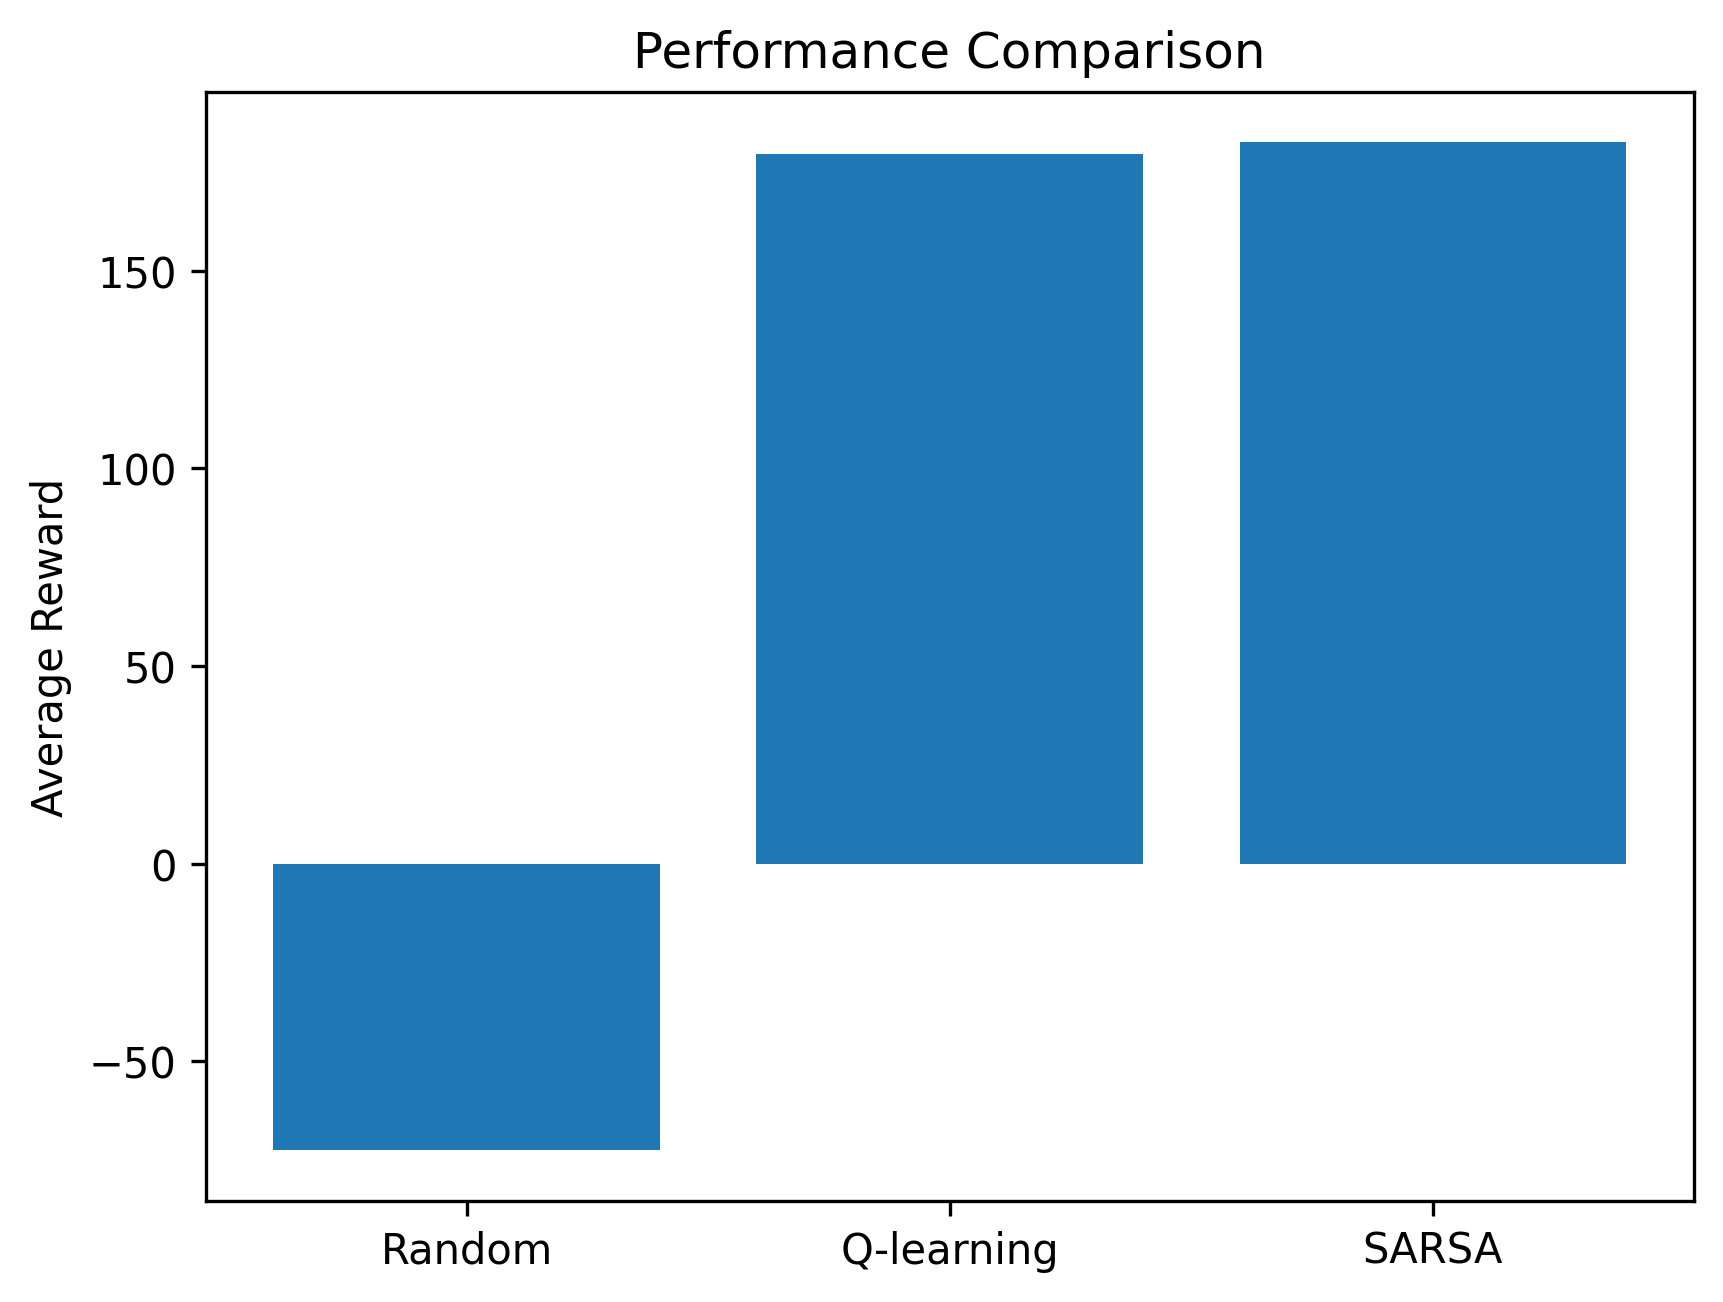
\includegraphics[width=0.75\textwidth]{performance_comparison.png}
    \caption{Confronto della reward media tra gli agenti.}
    \label{fig:performance_comparison}
\end{figure}

\FloatBarrier
L’agente casuale ottiene una reward media fortemente negativa, poiché tende a collidere rapidamente con il fantasma senza raccogliere quantità significative di cibo.

Gli agenti Q-Learning e SARSA ottengono invece reward medie elevate, dimostrando di aver appreso strategie efficaci.

\section{Confronto del numero di cibi raccolti}

La Figura~\ref{fig:food_comparison} confronta il numero medio di cibi raccolti.

\begin{figure}[H]
    \centering
    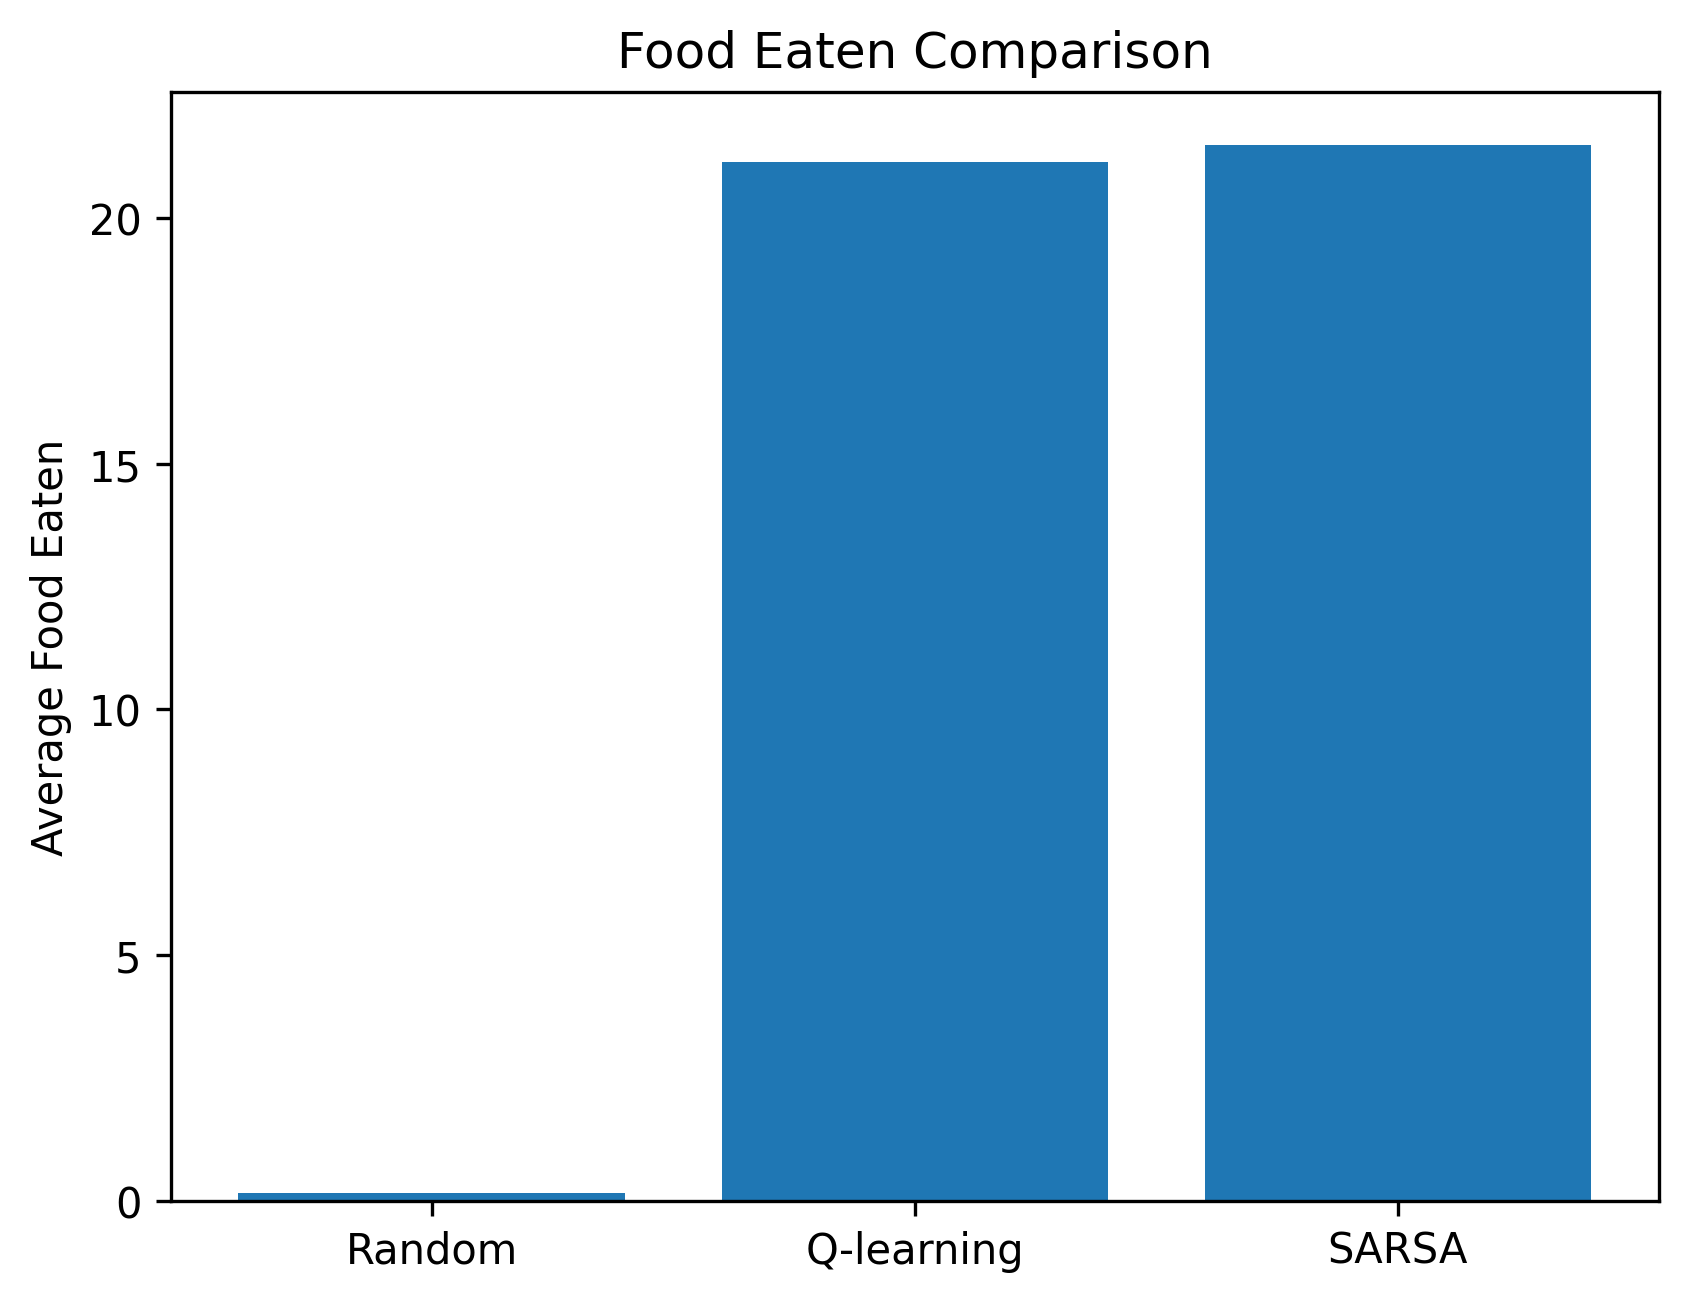
\includegraphics[width=0.75\textwidth]{food_comparison.png}
    \caption{Confronto del numero medio di cibi raccolti.}
    \label{fig:food_comparison}
\end{figure}
\FloatBarrier
Gli agenti addestrati riescono a raccogliere una quantità molto maggiore di cibo rispetto all’agente random. Questo comportamento indica che gli algoritmi hanno appreso politiche in grado di raggiungere rapidamente gli obiettivi presenti nell’ambiente.

\section{Confronto della sopravvivenza}

La Figura~\ref{fig:steps_comparison} mostra il numero medio di step sopravvissuti.

\begin{figure}[H]
    \centering
    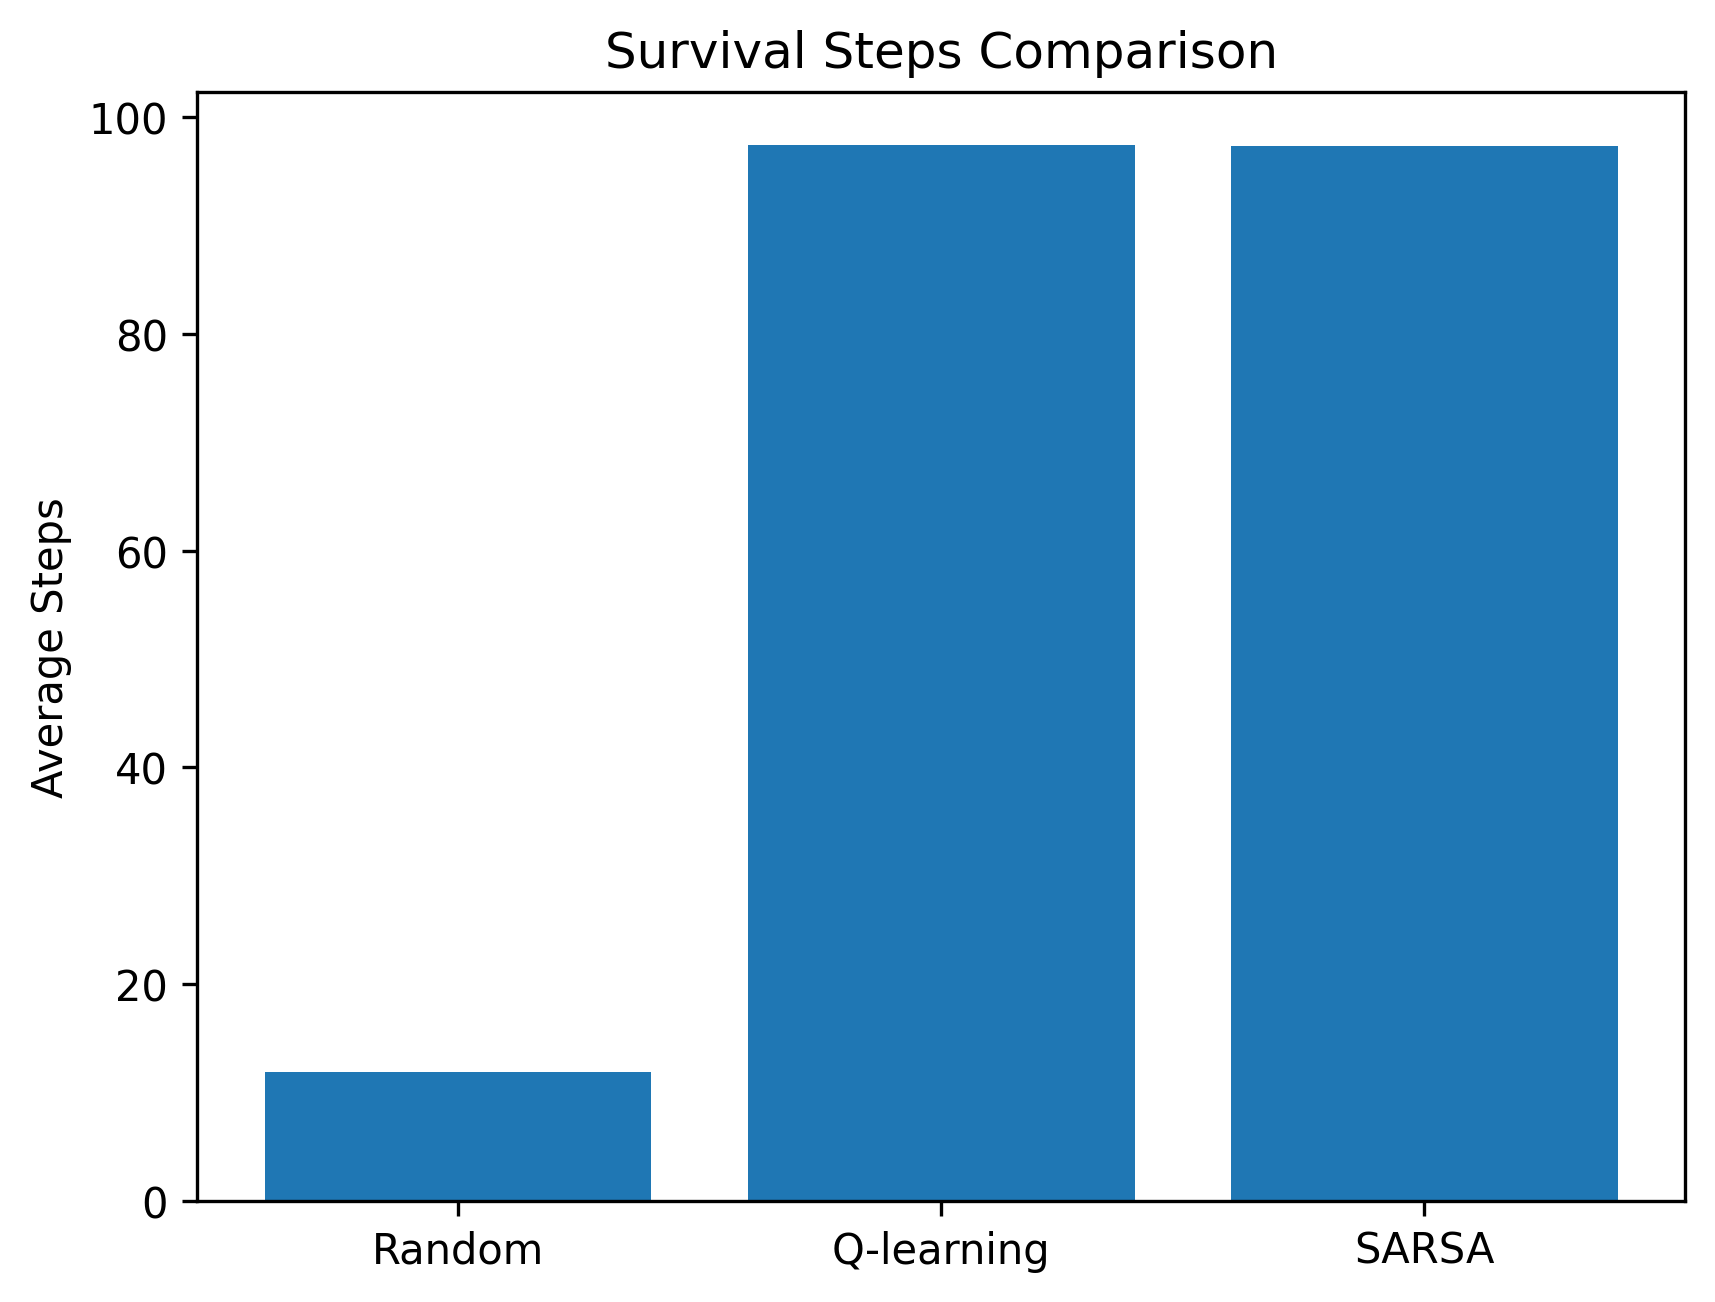
\includegraphics[width=0.75\textwidth]{steps_comparison.png}
    \caption{Confronto del numero medio di step sopravvissuti.}
    \label{fig:steps_comparison}
\end{figure}
\FloatBarrier
L’agente casuale sopravvive mediamente per pochi step, mentre gli agenti RL riescono quasi sempre a raggiungere il limite massimo di 100 step per episodio.

Questo risultato suggerisce che gli agenti hanno imparato strategie efficaci per evitare il fantasma.

\section{Confronto del collision rate}

La Figura~\ref{fig:collision_comparison} mostra il tasso di collisione con il fantasma.

\begin{figure}[H]
    \centering
    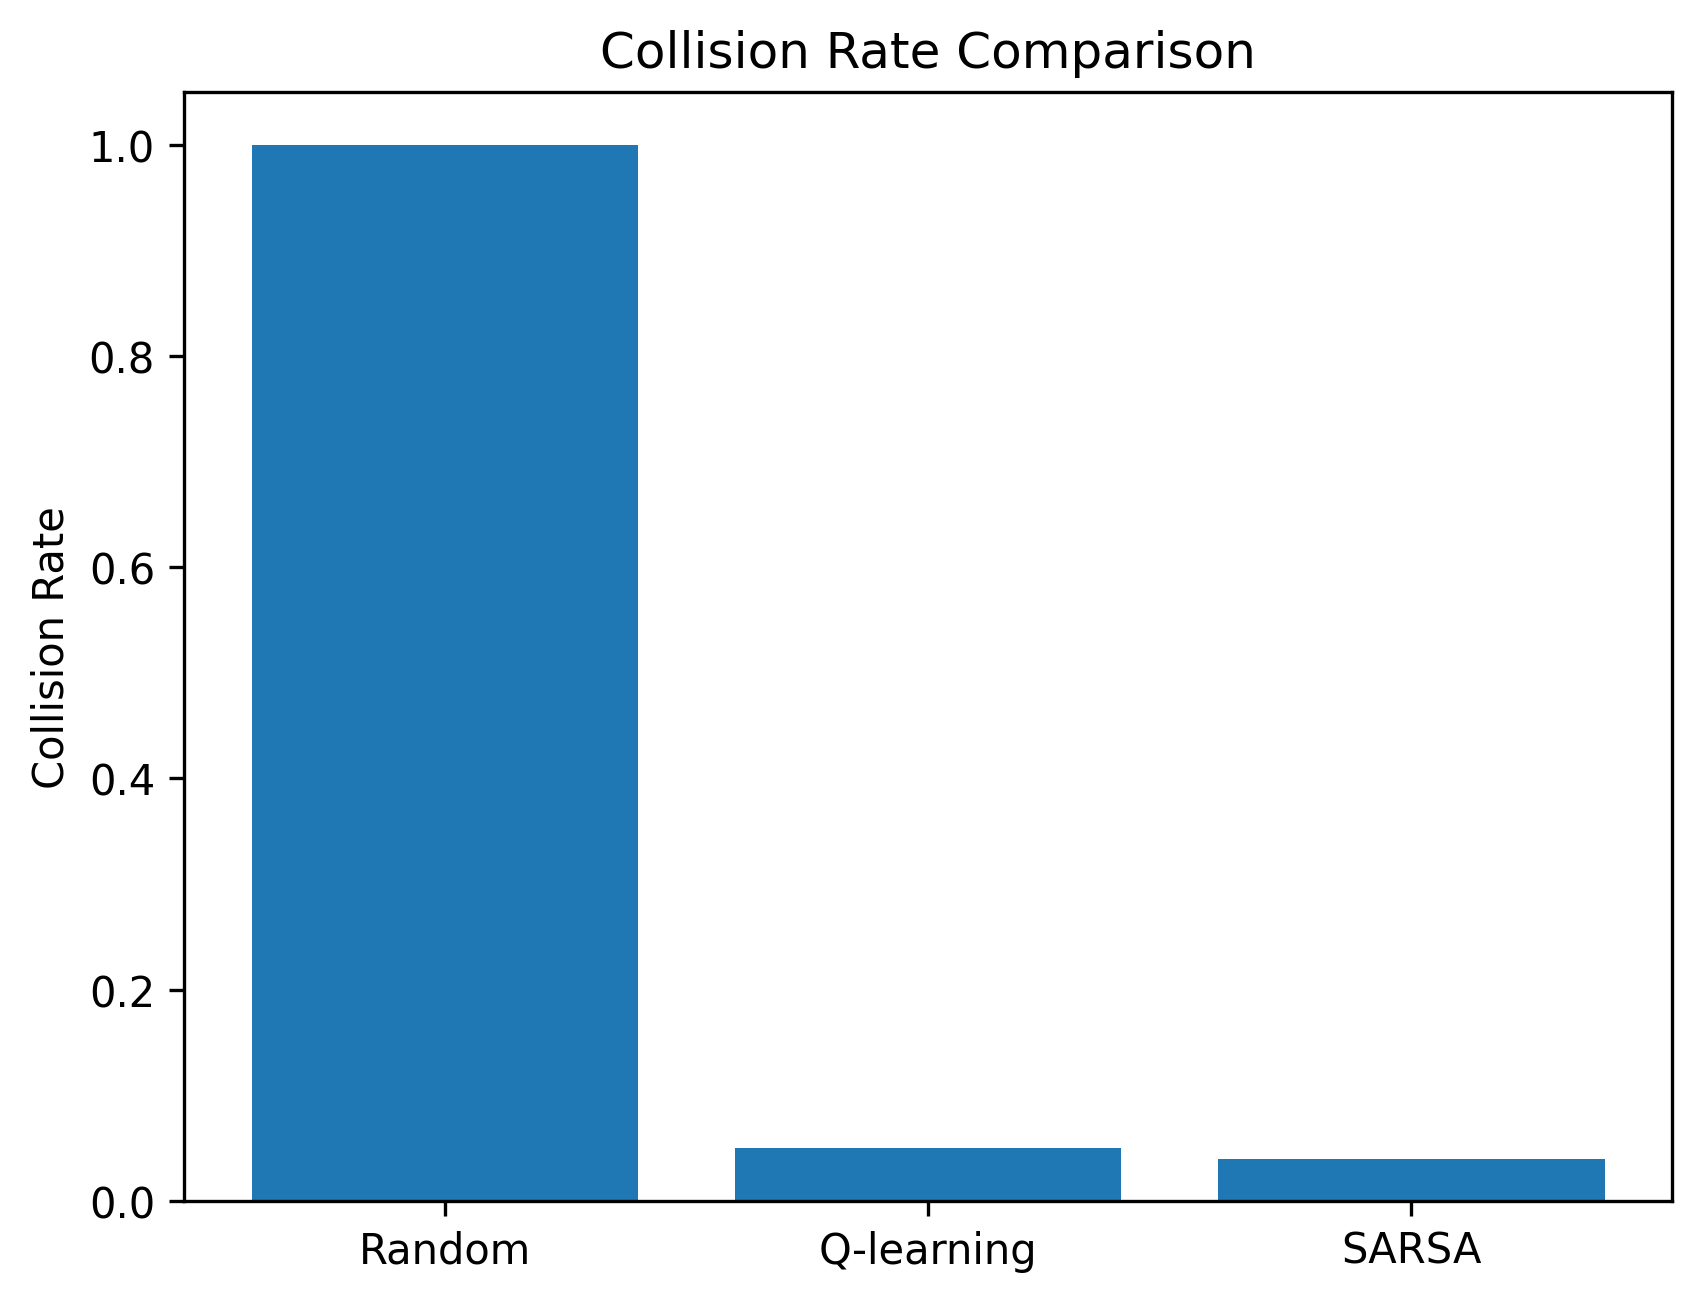
\includegraphics[width=0.75\textwidth]{collision_comparison.png}
    \caption{Confronto del collision rate tra gli agenti.}
    \label{fig:collision_comparison}
\end{figure}
\FloatBarrier
L’agente casuale presenta un collision rate pari al 100\%, indicando che termina praticamente tutti gli episodi entrando in collisione con il fantasma.

Al contrario, Q-Learning e SARSA mantengono collision rate molto bassi, confermando la capacità di apprendere comportamenti di sopravvivenza efficaci.

\section{Confronto tra Q-Learning e SARSA}

Il confronto tra i due algoritmi evidenzia differenze coerenti con la teoria del Reinforcement Learning.

Q-Learning ottiene prestazioni leggermente superiori in termini di reward media, numero di cibi raccolti e collision rate. Questo comportamento è coerente con la natura off-policy dell’algoritmo, che tende a privilegiare strategie più aggressive e orientate alla massimizzazione della reward futura.

SARSA, invece, mostra un comportamento leggermente più prudente. Poiché aggiorna i valori Q considerando le azioni realmente selezionate dalla politica corrente, comprese quelle esplorative, tende a sviluppare strategie più conservative.

Nonostante queste differenze, entrambi gli algoritmi riescono ad apprendere politiche efficaci e a superare nettamente l’agente casuale.

\chapter{Discussione dei Risultati}

L’analisi dei risultati ottenuti mostra che gli algoritmi di Reinforcement Learning implementati riescono ad apprendere strategie efficaci all’interno dell’ambiente Pac-Man sviluppato.

Fin dalle prime fasi del training si osserva un miglioramento progressivo della reward media, accompagnato da un aumento del numero di cibi raccolti e da una riduzione delle collisioni con il fantasma. Questo comportamento conferma che gli agenti riescono progressivamente a comprendere la struttura dell’ambiente e a selezionare azioni sempre più vantaggiose.

\section{Comportamento dell’agente casuale}

L’agente casuale presenta prestazioni molto basse in tutte le metriche considerate. Il collision rate pari al 100\% indica che l’agente termina praticamente ogni episodio entrando in collisione con il fantasma.

La reward media negativa e il numero ridotto di step sopravvissuti mostrano chiaramente che un comportamento puramente casuale non è sufficiente per affrontare efficacemente il problema.

Questo risultato rappresenta un utile baseline per valutare l’effettiva capacità di apprendimento degli algoritmi RL.

\section{Apprendimento degli agenti RL}

Sia Q-Learning sia SARSA riescono a sviluppare strategie efficaci. Gli agenti imparano progressivamente a:

\begin{itemize}
    \item evitare il fantasma;
    \item minimizzare i movimenti inutili;
    \item raggiungere rapidamente il cibo;
    \item sopravvivere per un numero elevato di step.
\end{itemize}

L’elevata reward media ottenuta e il basso collision rate confermano la qualità delle politiche apprese.

I grafici di training mostrano inoltre che, nonostante la presenza di rumore nella reward dei singoli episodi, la media mobile presenta un andamento crescente abbastanza stabile. Questo comportamento è tipico degli ambienti stocastici nel Reinforcement Learning.

\section{Interpretazione del Q-value}

Durante il training è stato monitorato anche l’andamento del valore Q associato allo stato iniziale dell’episodio. Tale valore mostra una crescita progressiva nel corso degli episodi, indicando che la Q-table attribuisce stime sempre più elevate della reward futura attesa.

Tuttavia, il Q-value non converge perfettamente a un valore costante. Questo comportamento è plausibile e coerente con la struttura dell’ambiente utilizzato.

Infatti:

\begin{itemize}
    \item la posizione del cibo varia casualmente a ogni episodio;
    \item il fantasma utilizza una politica di movimento parzialmente casuale;
    \item la politica $\epsilon$-greedy mantiene una componente di esplorazione durante tutto il training.
\end{itemize}

Di conseguenza, lo stato iniziale non è identico in ogni episodio e le stime della reward futura rimangono soggette a variazioni.

Per questo motivo, il Q-value deve essere interpretato principalmente come un indicatore qualitativo dell’apprendimento della Q-table, piuttosto che come una misura esatta della convergenza dell’algoritmo.

\section{Differenze tra Q-Learning e SARSA}

Le differenze osservate tra Q-Learning e SARSA risultano coerenti con la teoria.

Q-Learning ottiene prestazioni leggermente superiori in termini di reward media e collision rate. Questo comportamento deriva dalla natura off-policy dell’algoritmo, che aggiorna i valori Q assumendo sempre l’azione ottimale nello stato successivo.

SARSA, essendo on-policy, aggiorna invece i valori Q considerando le azioni realmente selezionate dalla politica corrente. Di conseguenza, tende a sviluppare strategie più conservative e leggermente meno aggressive.

Nel contesto del progetto, entrambe le strategie si sono comunque dimostrate efficaci.

\section{Limiti del progetto}

Nonostante i risultati positivi, il progetto presenta alcune limitazioni.

L’ambiente utilizzato è relativamente piccolo e completamente osservabile. Inoltre, la Q-table cresce rapidamente all’aumentare della dimensione dello spazio degli stati, rendendo gli approcci tabulari poco scalabili per ambienti più complessi.

Un ulteriore limite riguarda l’utilizzo di un valore di $\epsilon$ costante durante tutto il training. L’introduzione di una strategia di epsilon decay potrebbe migliorare ulteriormente la convergenza degli algoritmi.

Infine, i risultati sono stati ottenuti eseguendo un singolo training per algoritmo. In contesti sperimentali più avanzati sarebbe opportuno effettuare più esecuzioni con seed differenti e analizzare media e deviazione standard delle metriche ottenute.


\chapter{Conclusioni}

In questo progetto è stato sviluppato un ambiente semplificato ispirato al gioco Pac-Man per analizzare il comportamento di algoritmi di Reinforcement Learning tabulare. In particolare, sono stati implementati e confrontati due algoritmi classici: Q-Learning e SARSA.

L’ambiente progettato include elementi di stochasticità dovuti sia alla generazione casuale del cibo sia al comportamento parzialmente casuale del fantasma. Questo ha reso il problema sufficientemente dinamico da richiedere strategie adattive da parte degli agenti.

I risultati ottenuti mostrano chiaramente che entrambi gli algoritmi di Reinforcement Learning riescono ad apprendere politiche efficaci. Rispetto all’agente casuale, Q-Learning e SARSA ottengono reward medie significativamente più elevate, raccolgono un numero maggiore di cibi e riducono drasticamente il tasso di collisione con il fantasma.

L’analisi dei grafici di training conferma inoltre la presenza di apprendimento durante gli episodi. Nonostante il rumore presente nelle reward e nei valori Q, dovuto alla natura stocastica dell’ambiente, il trend generale evidenzia un miglioramento progressivo delle performance.

Il confronto tra Q-Learning e SARSA ha permesso di osservare differenze coerenti con la teoria del Reinforcement Learning. Q-Learning ha mostrato un comportamento leggermente più aggressivo e orientato alla massimizzazione della reward, mentre SARSA ha evidenziato una strategia più prudente e conservativa.

Nel complesso, il progetto dimostra come anche algoritmi tabulari relativamente semplici siano in grado di apprendere comportamenti efficaci in ambienti dinamici e non completamente deterministici.

Possibili sviluppi futuri includono:

\begin{itemize}
    \item utilizzo di strategie di epsilon decay;
    \item esecuzione di più training con seed differenti;
    \item introduzione di ambienti più complessi;
    \item utilizzo di Deep Reinforcement Learning;
    \item aggiunta di più fantasmi o mappe di dimensioni maggiori.
\end{itemize}

Questi miglioramenti permetterebbero di estendere ulteriormente il progetto verso scenari più realistici e complessi.

\begin{thebibliography}{9}

\bibitem{slides}
Francesco Pupo,
\textit{Lecture Slides - Intelligent Systems for Robotics},
University of Calabria, Academic Year 2025--2026.

\bibitem{sutton}
Richard S. Sutton and Andrew G. Barto,
\textit{Reinforcement Learning: An Introduction},
Second Edition,
MIT Press, 2015.

\bibitem{Pygame}
Pygame Documentation,
\url{https://www.pygame.org/docs/}

\bibitem{NumPy}
NumPy Documentation,
\url{https://numpy.org/doc/}

\bibitem{Matplotlib}
Matplotlib Documentation,
\url{https://matplotlib.org/stable/}

\end{thebibliography}


\end{document}